% ********** Chapter 4 **********
\chapter{Solution}
\label{sec:Solution}

There are two kind of connection solution of the core of Web Call, the Relay Call and Third Party Call. The different between them is the way they handle media stream.

The Relay Call Controller works as a back-to-back agent and forwards media streams, while Third Party Call Controller only establishes connections by sending out SIP messages and it does not handles any streams itself. 

\section{Relay Call}
\label{sec:Solution:RelayCall}

\begin{figure}[!hbtp]
\centering
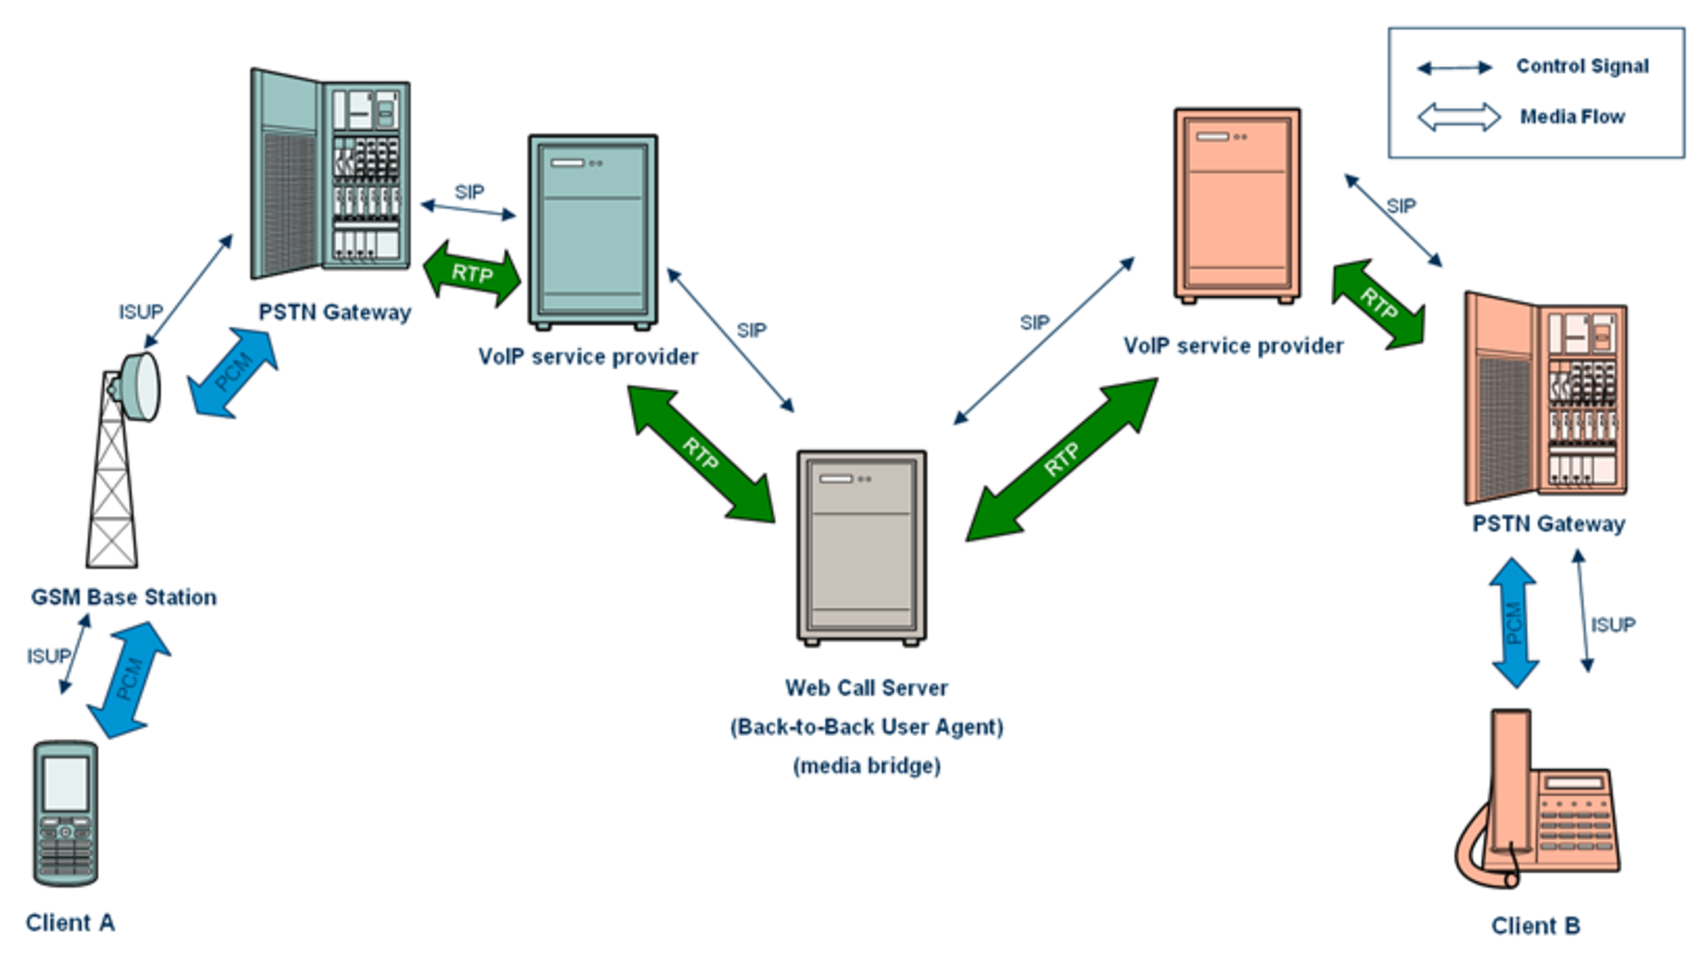
\epsfig{file=chap04/resources/the_signal_and_media_flow_of_relay_call, width=5.34in}
\caption{The signal and media flow of Relay Call}
\label{fig:TheSignalAndMediaFlowOfRelayCall}
\end{figure}

The signal and media flow of Relay Call is shown in Figure \ref{fig:TheSignalAndMediaFlowOfRelayCall}. In this scenario, the Web Call Example Application acts as a back-to-back user agent. It sets up the connection and forwards the media stream. It can be seen from the picture that both signal and media are handled by Web Call Server. When it starts, it try to call client A. After it establishes a session with client A, it will try to call client B and also establish a session with client B. After that, it will work as a media stream bridge and forward media stream from client A to B, as well as from client B to A.


Follow document shows three call flows that presents the typical three different use cases of SIP controller in a phone-to-phone logic environment.

\subsection{Normal Case of Relay Call}
\label{sec:Solution:RelayCall:NormalCaseOfRelayCall}

The basic case flow is shown in Figure \ref{fig:NormalCaseOfRelayCall}. The controller first sends an INVITE to A. A's phone rings, and A answers. This results in a 200 OK that is sent to session initiator, controller. The controller needs to send the ACK. This part is the typical SIP session setup steps. After the session between controller and client A has been established, controller starts to send ring tone to client A, indicating that it is waiting for B to answer the phone. Once the controller receives a 200 OK from client A, it start another session initiation with client B by sending INVITE to B. After B answers the phone, controller receives 200 OK from client B. It will stop sending ring tone to A, and start RTP packets proxy between A and B.

\begin{figure}[!hbtp]
\centering
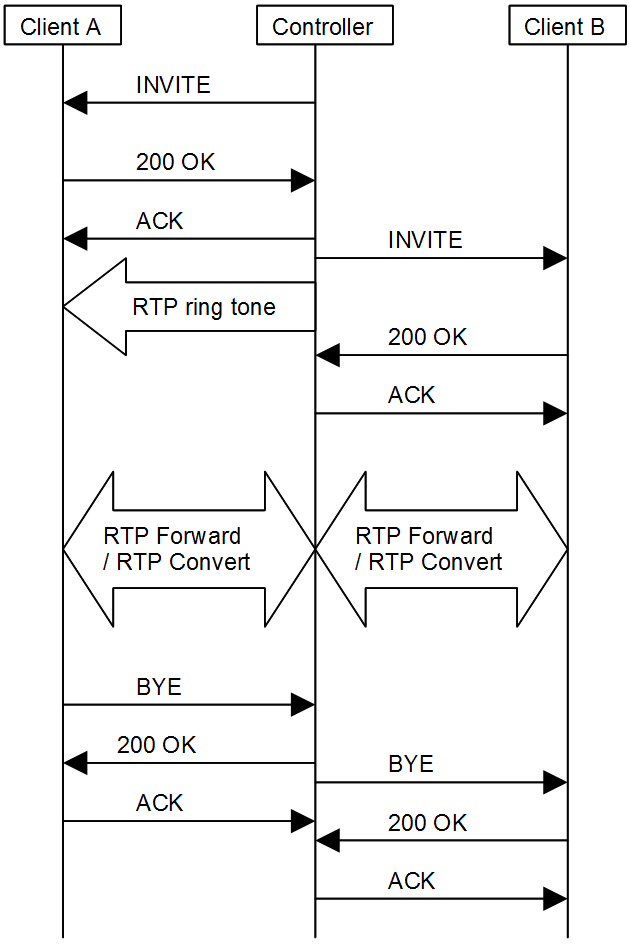
\epsfig{file=chap04/resources/normal_case_of_relay_call, width=5.34in}
\caption{Normal Case of Relay Call}
\label{fig:NormalCaseOfRelayCall}
\end{figure}

\subsection{Cancel Case of Relay Call}
\label{sec:Solution:RelayCall:CancelCaseOfRelayCall}

In the Cancel case which is shown in Figure \ref{fig:CancelCaseOfRelayCall}, the session initiation with client A is the same as normal case. While controller is waiting for client B to answer the phone, client A hangs up the phone. This results in a BYE to the controller. On receiving the BYE message, controller stops sending ring tone to A, and sends a CANCEL to B. The CANCEL request is used to cancel the INVITE request sent by the controller. When a SIP server receives a CANCEL request for an INVITE, but has not yet sent 200OK, would stop sending RING, and then respond to the INVITE with a specific error response 487 Request terminated. 

\begin{figure}[!hbtp]
\centering
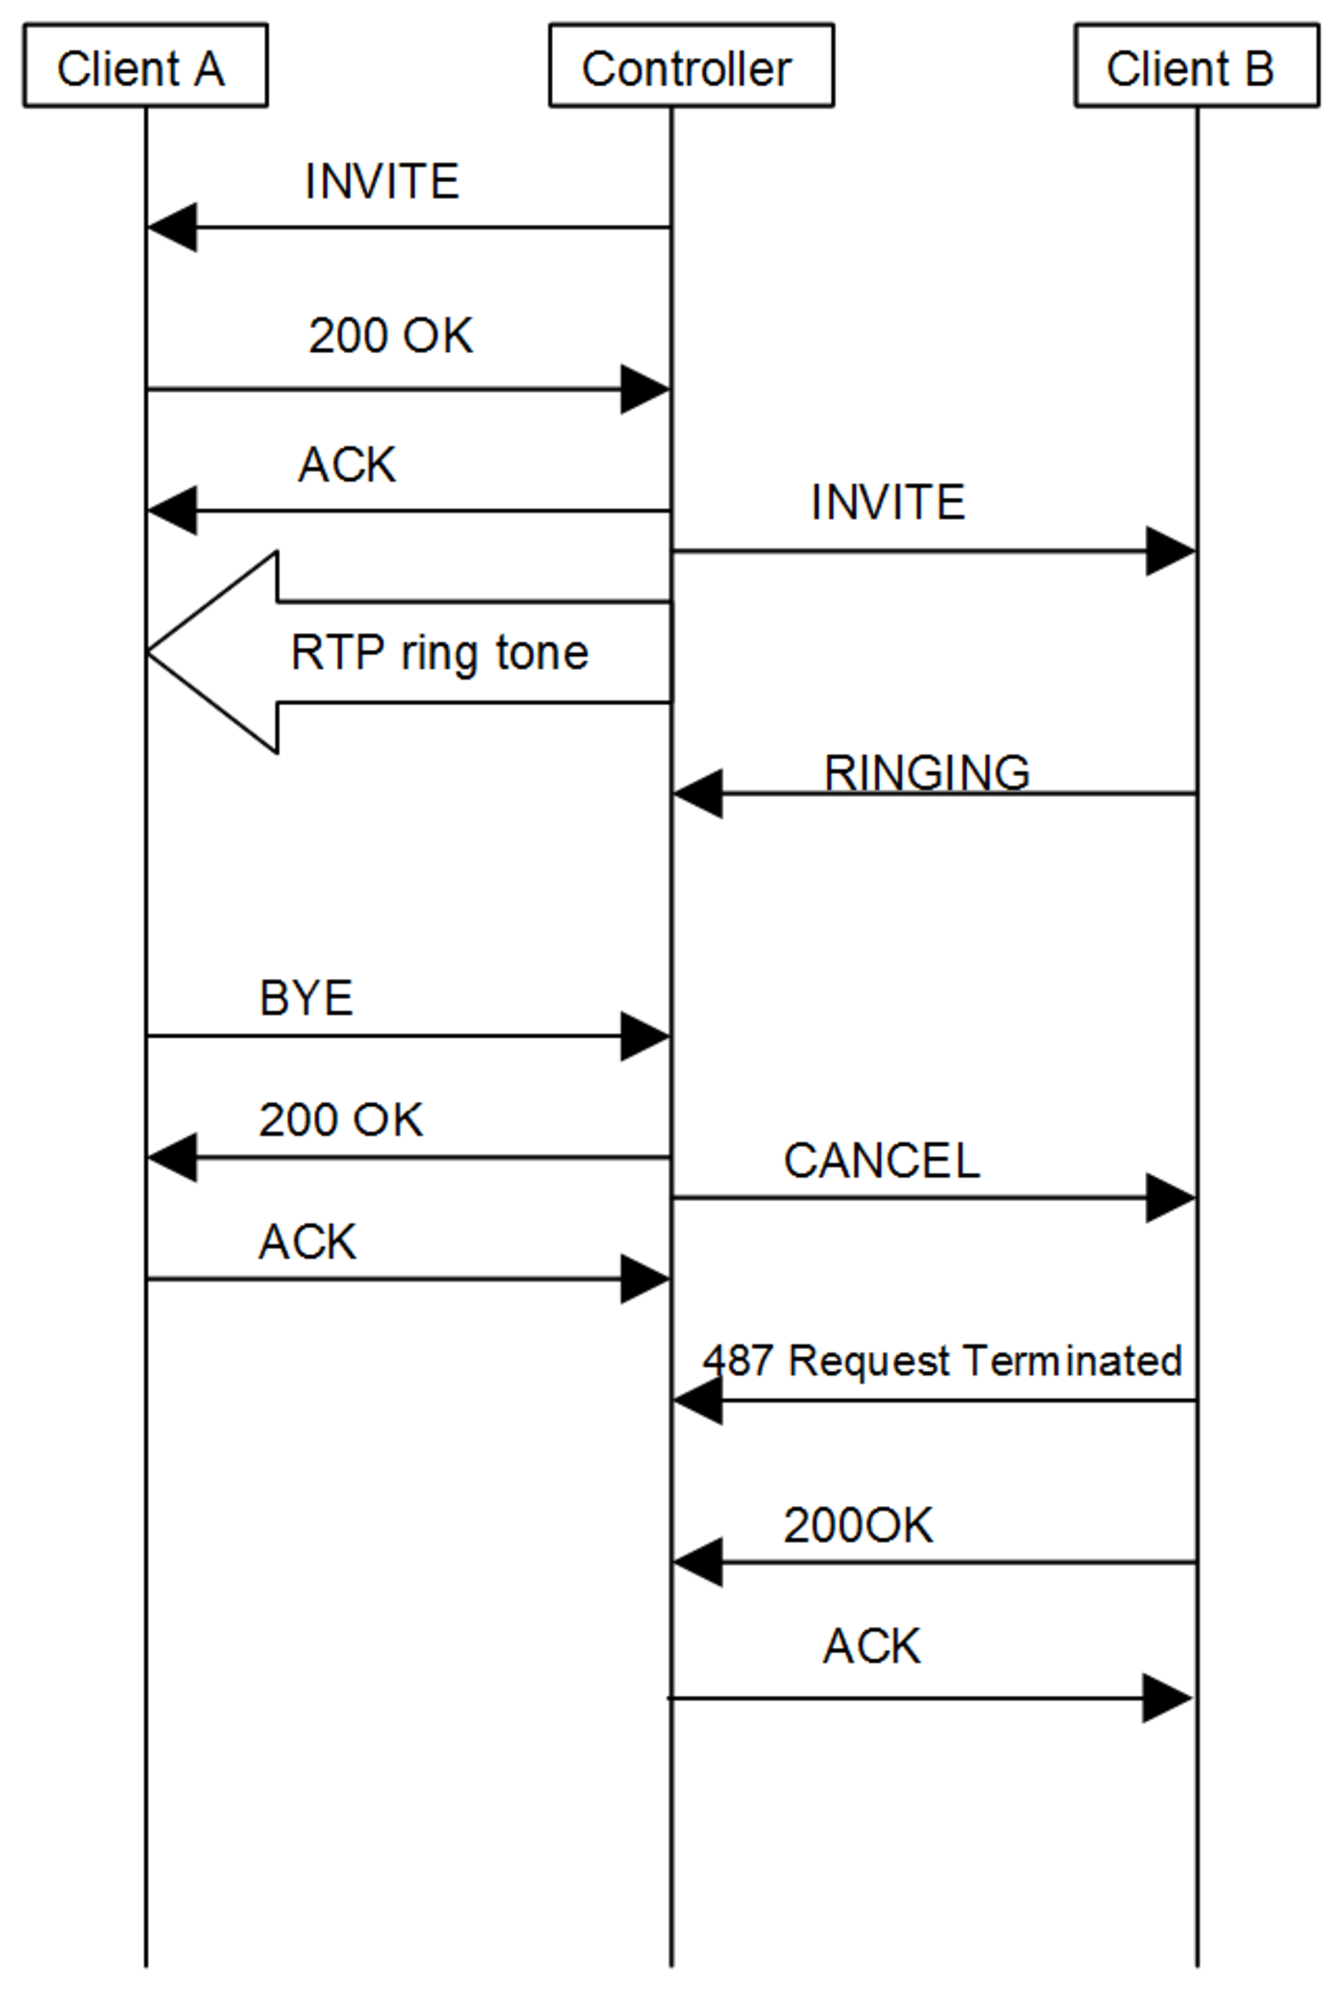
\epsfig{file=chap04/resources/cancel_case_of_relay_call, width=5.34in}
\caption{Cancel Case of Relay Call}
\label{fig:CancelCaseOfRelayCall}
\end{figure}


\subsection{Rejection Case of Relay Call}
\label{sec:Solution:RelayCall:RejectionCaseOfRelayCall}

In the rejection case which is shown in Figure \ref{fig:RejectionCaseOfRelayCall}, the session initiation with client A is the same as normal case. While controller is waiting for client B to answer the phone, it receives a 4xx message from B, for example, 486 Busy Here or 404 Not Found. At this situation, the controller will send an ACK to client B, stop sending the ring tone, and try to terminate the session with client A by sending a BYE message.  

\begin{figure}[!hbtp]
\centering
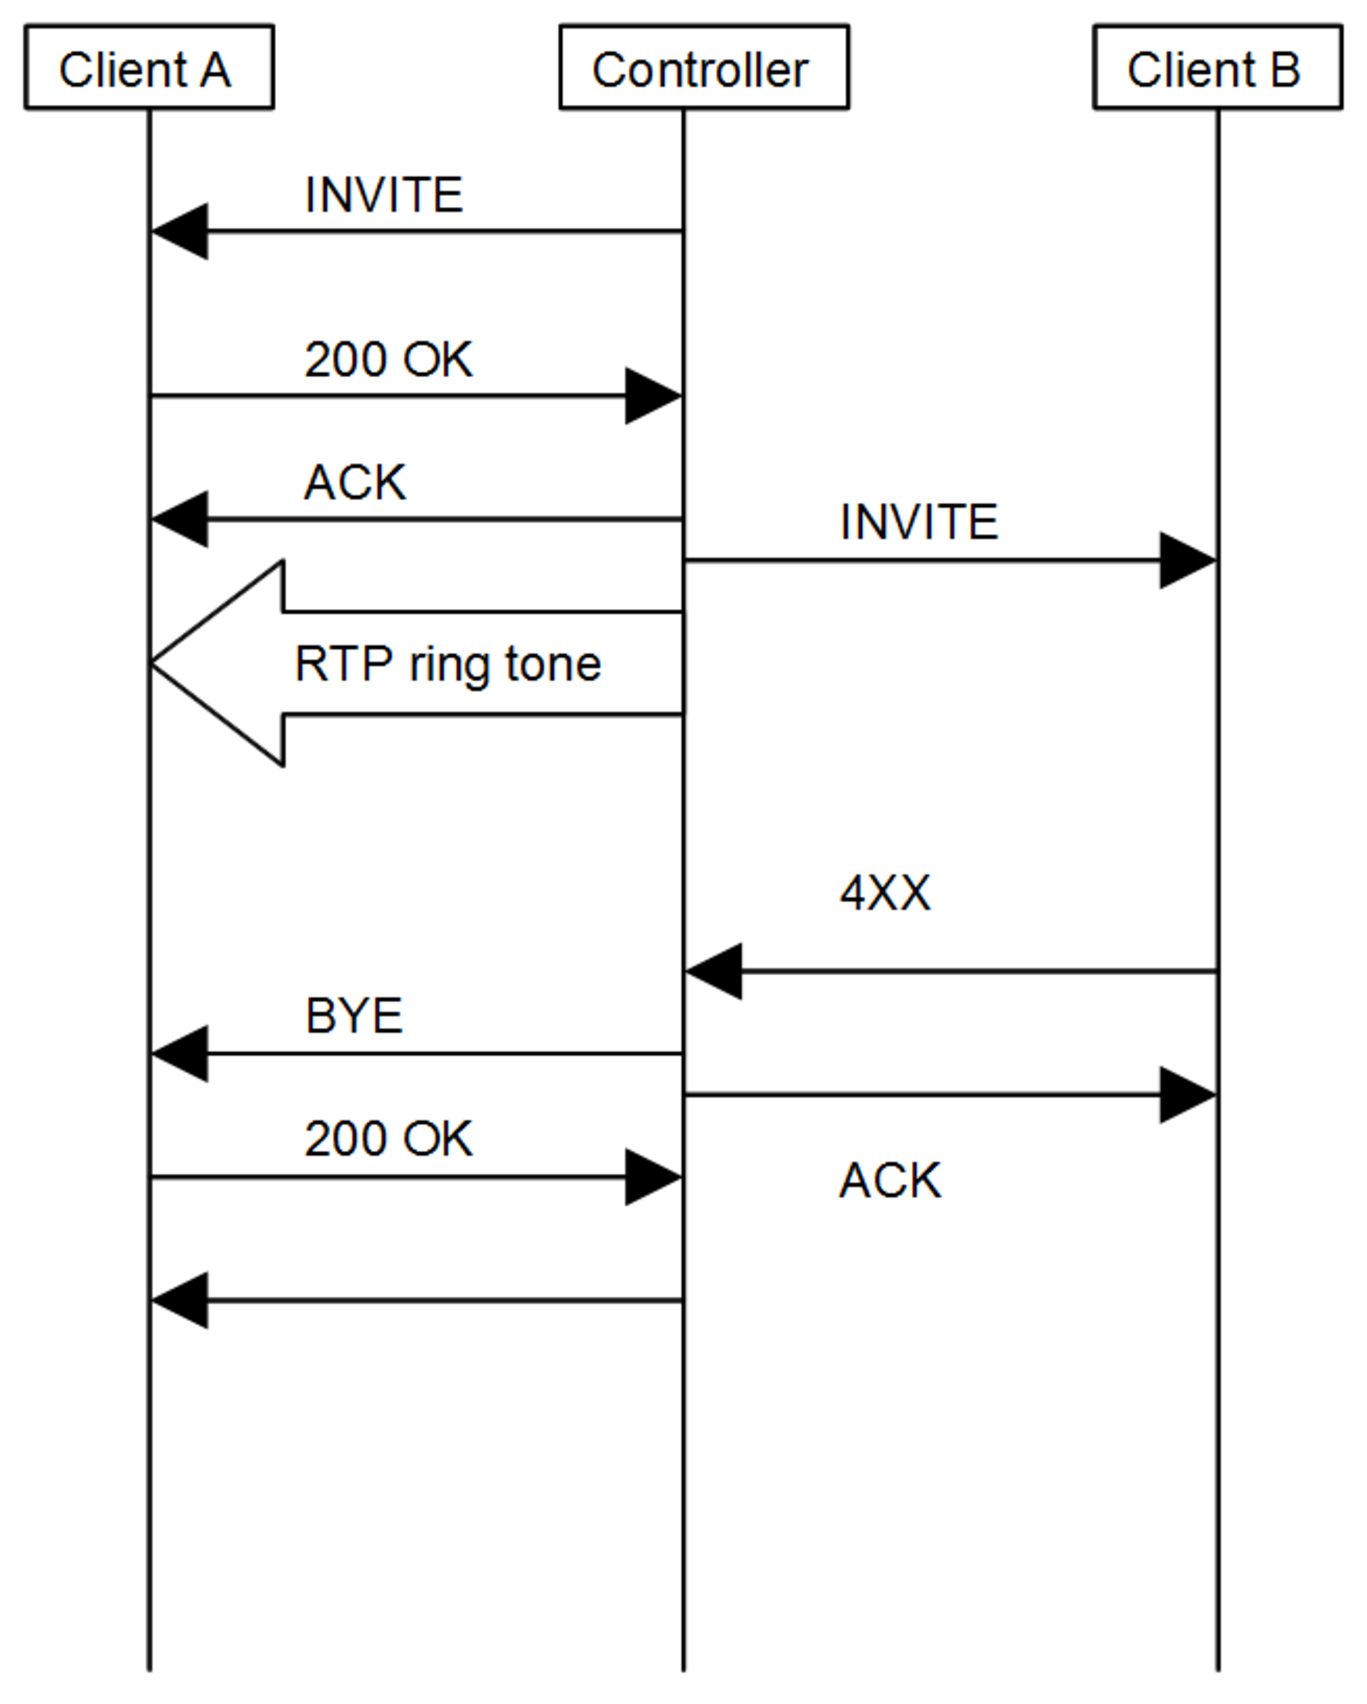
\epsfig{file=chap04/resources/rejection_case_of_relay_call, width=5.34in}
\caption{Rejection Case of Relay Call}
\label{fig:RejectionCaseOfRelayCall}
\end{figure}

\clearpage

\section{Third Party Call}
\label{sec:Solution:ThirdPartyCall}

In the traditional telephony context, third party call control allows one entity (which we call the controller) to set up and manage a communications relationship between two or more other parties. Third Party call control (referred as 3pcc) is often used for operator services (where an operator creates a call that connects two participants together) and for conferencing. The signal and media flow in third party call is show in Figure \ref{fig:TheSignalAndMediaFlowOf3pc} The advantage of third party call in Web Call is that the controller only need to handle message transfer and leaves the media flow for the ISP.

\begin{figure}[!hbtp]
\centering
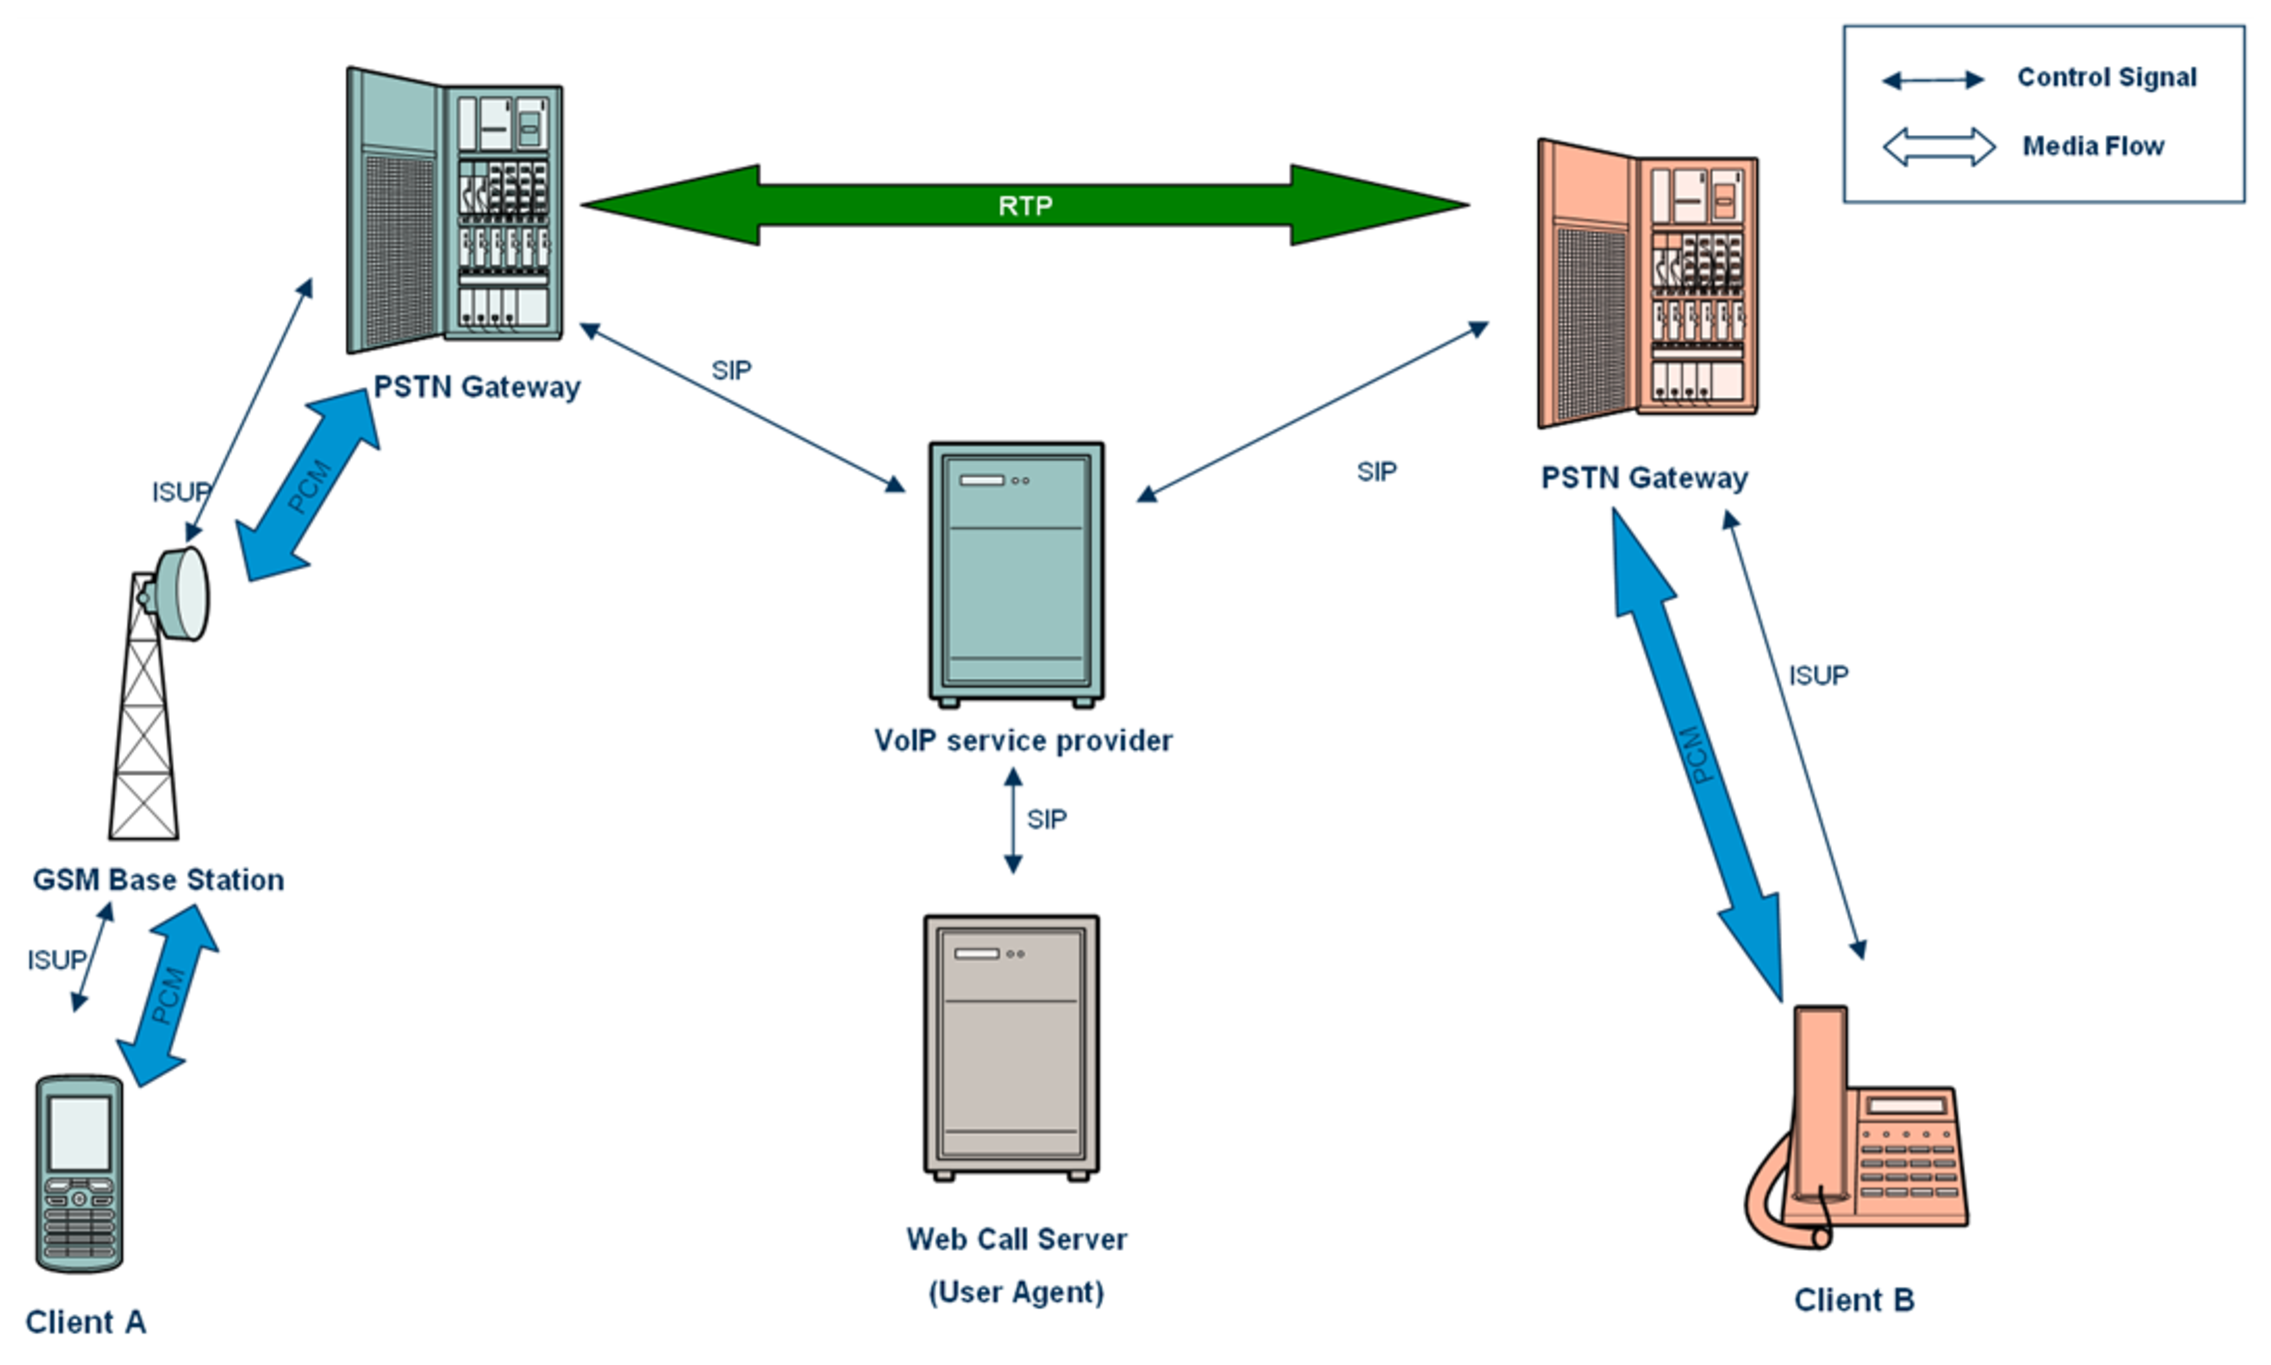
\epsfig{file=chap04/resources/the_signal_and_media_flow_of_3pc, width=5.34in}
\caption{The signal and media flow of Third Party Call}
\label{fig:TheSignalAndMediaFlowOf3pc}
\end{figure}




\subsection{Call Transfer}
\label{sec:Solution:ThirdPartyCall:CallTransfer}


\subsection{SDP Swap}
\label{sec:Solution:ThirdPartyCall:SDPSwep}

\subsection{Re-invite}
\label{sec:Solution:ThirdPartyCall:Re-invite}

\subsection{Web Client}
\label{sec:Solution:ThirdPartyCall:WebClient}


\section{Conclusion}
\label{sec:Solution:Conclusion}




% ********** End of chapter **********
